\documentclass{article}
\usepackage{graphicx} % Required for inserting images
\usepackage{listings}
\usepackage{caption}
\usepackage{subcaption}
\usepackage[style=apa, backend=biber]{biblatex}
\bibliography{references}


\title{Portrait Optimization via Deep Learning: A Framework for Context-Aware Photography Recommendations}
\author{Shriya Nair and Bucky Hayes}


\begin{document}

\maketitle

\section{Abstract}

The photo-aid portrait optimizer is an ongoing project to create a mobile application that detects multiple attributes of an image to influence the quality of professional photos through a Machine Learning Approach. This report describes my approach to training and testing models on the Wider Facial Landmarks in the Wild (WFLW) dataset to detect influential attributes that affect the quality of a portrait image. It details the stages of the project, challenges with each stage, findings, and future work. 

\section{Project Overview}

The current product includes 6 separate models corresponding to the blur, occlusion, make-up, expression, illumination, and pose values in a given portrait and categorizes them with the labels '0' and '1'. '0' indicates that the factor is normal, while '1' indicates that it is extreme or unusual. For example, if a picture is said to have an occlusion value of 1 and an illumination value of 1, it indicates that there is something blocking or occluding the person and that the photo is either too bright or too dark. The models for each attribute vary slightly from each other in their learning rates to aid in optimization. While the training accuracies of all models were above 95.5\% (see Tabel 1 Below) the testing accuracies declined significantly for blur and illumination (see Figure 2). Further alterations to each model composition may be required in order to gain fully accurate models. 


\section{Development Process}

\subsection{Selecting a Dataset}

The WFLW (Wider Facial Landmarks in the Wild) dataset contains 10,000 image, 7,500 for training and 2,500 for testing. The dataset also contains annotations of 98 facial landmark coordinates, binary annotations of the blur, occlusion, make-up, expression, illumination, and pose values of each image, and bounding box annotations. The diversity in annotation data which could diversify my model by incorporating classification and recognition models appealed to me, and I chose the WFLW dataset as a starting point to gain experience in working with Convolutional Neural Nets. Overall, working with the binary attribute data of the WFLW dataset was an intuitive experience, and the simplification of subjective measuring of attributes into binary data allowed me to achieve my purpose of working with image classification at a base level. 

In order to obtain the annotation data into a workable file format, with assistance from my mentor Bucky Hayes, I developed a python script to parse the textual annotation data into a python dictionary and then parsed that into a csv file stored locally. Csv files were easy to work with and allowed for the dataset to be examined and manipulated easily.

\begin{figure}[h]
    \centering
    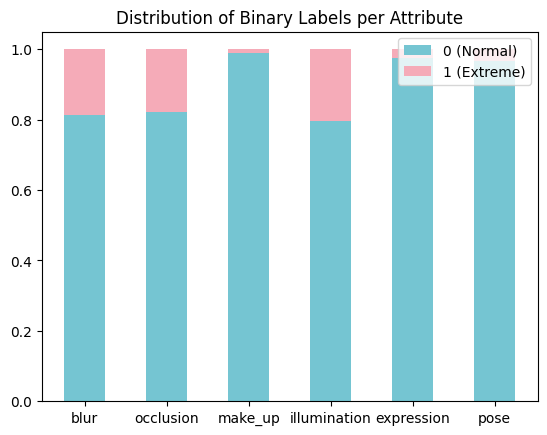
\includegraphics[width=0.8\linewidth]{Distro-of-binary-annotation-labels.png}
    \caption{Distribution of unique labels per attribute}
    \label{fig:enter-label}
\end{figure}
A challenge in working with the WFLW dataset was the imbalance of the set. As shown in the figure above, the class imbalance was significant and different for each of the attributes. To overcome this, I included a function in my training program to assign class weights to each 0/1 category to balance out the outcomes of the neural network so that the model is not biased after training and so it is simpler to measure the model using accuracy. 
\\


\subsection{Model Constants}
While the models varied from each other in learning rates and batch-sizes, the rest of each model was kept constant between the different attributes. This allowed me to get a better intuition for manipulating hyper-parameters and measuring the accuracy of the model. 
\\\\
Optimizer: Adam 
\\\\
Loss Function: Binary Crossentropy
\\\\
Model Layers: The model is a sequential model utilizing the Input, Dense, Flatten Dropout , DepthwiseConv2D , and MaxPooling2D layers from tensorflow.keras.models. The layers consist of 3 2D Depthwise Convolutional layers with kernel sizes of 3x3, and activation functions of ReLu to enable binary classification. The depthwise layers help in reducing the overall complexity of the neural net while preserving spatial data and maintaining most of the accuracy. After each Depthwise layer, there is a MaxPool layer with a pool size of 2x2- this allows for the model to limit dimensions and shorten the output from the Depthwise layers. One regular Convolutional 2D layer is included after one Depthwise and MaxPooling layer to increase dimensions and complexity of the model. In order to transfer the model into a one-dimensional object, the layers are Flattened and put through a Dense layer with 128 neurons and an activation function of ReLu. Then, a Dropout layer is implemented to rid the model of noise and further condense it. Finally, a dense layer with one output neuron and a sigmoid activation function determines the "0" or "1" attribute classification of the image. Below is the code that creates the model.



\begin{tiny}
\begin{lstlisting}

from tensorflow.keras.models import Sequential
from tensorflow.keras.layers import Input, Dense, Flatten, Dropout, DepthwiseConv2D, MaxPooling2D

model = tf.keras.Sequential([
    tf.keras.layers.Rescaling(1./255, input_shape=(96, 96, 3)),

    tf.keras.layers.DepthwiseConv2D(kernel_size=(3, 3), activation='relu', padding='same'),
    tf.keras.layers.MaxPooling2D(pool_size=(2, 2)),

    tf.keras.layers.Conv2D(32, (1, 1), activation='relu', padding='same'), 
    tf.keras.layers.DepthwiseConv2D(kernel_size=(3, 3), activation='relu', padding='same'),
    tf.keras.layers.MaxPooling2D(pool_size=(2, 2)),

    tf.keras.layers.DepthwiseConv2D(kernel_size=(3, 3), activation='relu', padding='same'),
    tf.keras.layers.MaxPooling2D(pool_size=(2, 2)),

    tf.keras.layers.Flatten(),
    tf.keras.layers.Dense(128, activation='relu'),
    tf.keras.layers.Dropout(0.5),

    tf.keras.layers.Dense(1, activation='sigmoid')  # Binary classification

])

\end{lstlisting}
\end{tiny}


\subsection{Model Training} 
Training the model involved many experimental conditions and manipulations. This section lists a log of findings from functions that inspected different conditions.
\\

1. Running All Attributes: The initial approach that I took to training my model was to run all the attributes on the same model in succession. On the first run through, I noticed a pattern of decreasing accuracy on each attribute. To ensure that the runs of separate attributes were not effecting each other, I reversed the attributes to run from pose to blur rather than blur to pose and plotted the accuracies as in the table below: 
\begin{figure}[h]
    \centering
    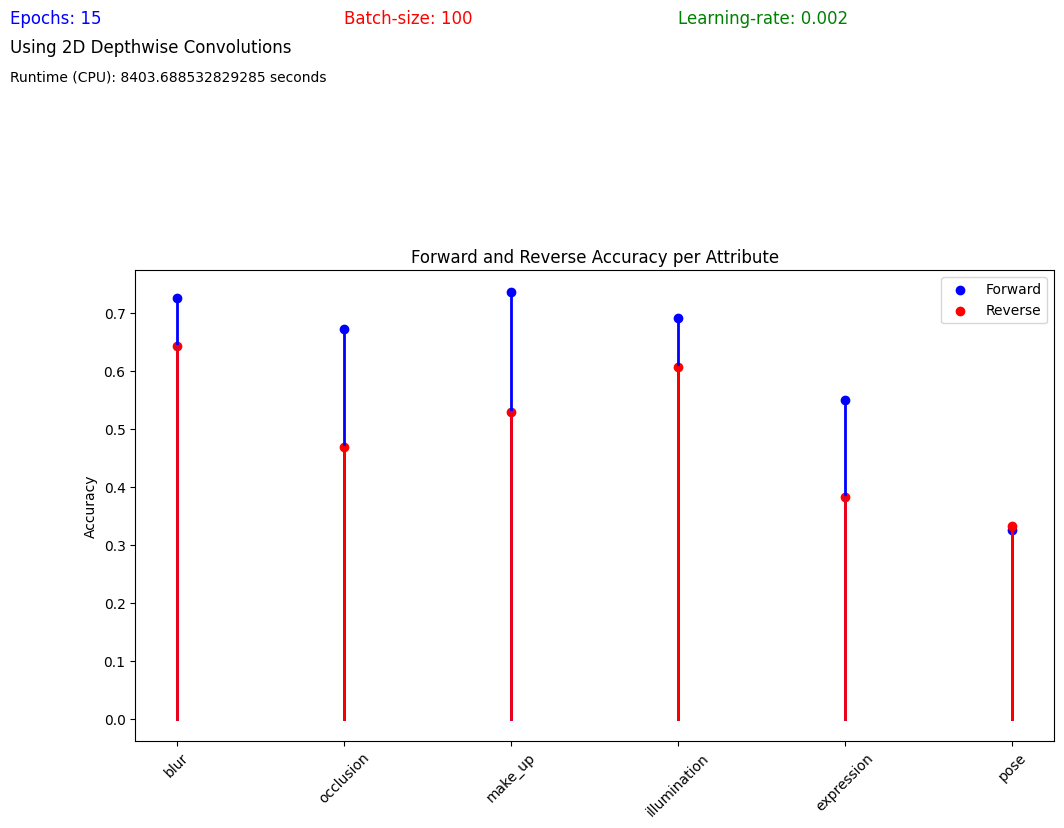
\includegraphics[width=0.5\linewidth]{15-epoch-fvr3.png}
    \caption{Forward vs Reverse Attribute Parsing}
    \label{fig:placeholder}
\end{figure} 
This showed that there was no clear decline over the models, as the reversed model shown in red did not show any sign of decrease. However, the pattern in the differences in success of the separate attributes showing consistent success of the blur and illumination accuracies suggested that the model was more suitable to specific attributes. This prompted the creating of six separate models for each attribute: each differing in learning rates to observe the relationship between hyper-parameters and the model. 

2. Separate Neural Networks: The second stage of training was to find the optimal hyperparameter values for each attribute. My approach was to find the rates manually.  My starting point was the previously measured accuracy of each attribute from the initial run- in which the learning rate was 0.0028. As an example of my optimization process, for the attribute make up, the accuracy was decent when the learning rate was near 0.0028 but the model was not improving past 95\% even with its gradual increase, so I then increased my learning rate to 0.0035, which resulted in the model over-training by not improving after 3/4 of the model. By adjusting the rate back to 0.003, I was able to reach my optimal accuracy of 99.1\% for make up. For batch size, the only batch size that was manipulated was that of occlusion. I reduced the batch size of the occlusion by 50\% in order for my model to increase in accuracy from around 90\% while using 100 as my batch size to 95\%. I only manipulated batch size for this single attribute in order to limit changes between the models due to the necessity of increasing accuracy.  While using algorithms such as Bayesian Optimization may have been more strategic to optimizing the hyper-parameters, manipulating the specific parameters manually gave me a better intuition on how each aspect changes the accuracy and rates of loss and was key in my learning of Neural Networks.

3. Multiple Runs: Another function that I created was to run the optimized model for a specific attribute multiple times within the same runtime and compare its speed to the result in which the model ran by increasing the number of epochs to the same number as with the multiple runs. 


\begin{figure}[h!]
  \centering
  \begin{subfigure}[b]{0.45\textwidth}
    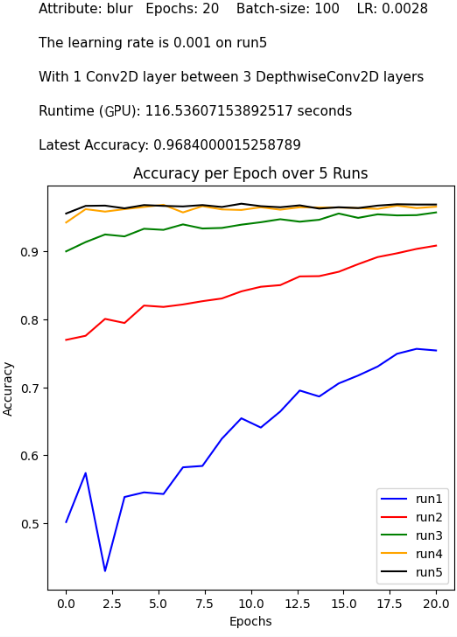
\includegraphics[width=\textwidth]{blururur.png}
    \caption{Ran 5 times (20 epochs)}
  \end{subfigure}
  \hfill
  \begin{subfigure}[b]{0.45\textwidth}
    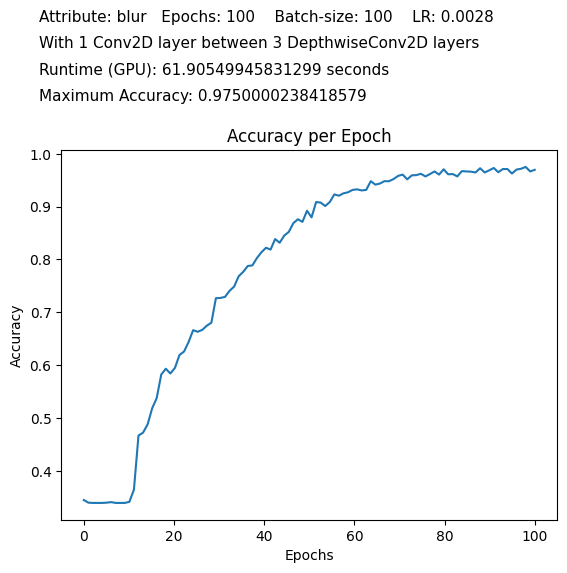
\includegraphics[width=\textwidth]{BLUR1.png}
    \caption{Ran once (100 epochs)}
  \end{subfigure}
  \caption{Running 5 times vs Running 1 time for equal number of total epochs}
\end{figure}

This plot was interesting in visualizing how my model retained its accuracy after each of its runs but increased gradually in an almost linear fashion each time rather than increasing logarithmically as in the single run with more epochs. The asymptotic behavior of the single run model as it approaches 100\% relates to how the slope of the lines of each run in the 5 time plot decrease in steepness each time until the final run almost matches in slope to its previous run, an indicator of the loss becoming minimized.
\\

Overall, through the model training process, I was able to study different aspects of a neural network, create comparisons, and gain a better intuition on how I can manipulate and work with them. The majority of my programming took place in this stage, and I was able to gain confidence in manipulating a neural net with each challenge that I overcame. The table below summarizes my results from the training process.

% Requires: \usepackage{multirow}
\begin{table}[h]
    \centering
    \begin{tabular}{|c|c|c|c|c|c|c|}
        \hline
        & Blur & Occlusion & Make Up & Expression & Illumination & Pose \\ \hline
        Accuracy & 97.3\% & 95.5\% & 99.1\% & 98.2\% & 98.9\% & 98.4\% \\ \hline
        Learning Rate & 0.0028 & 0.003285 & 0.003 & 0.0055 & 0.005 & 0.005 \\ \hline
        Batch-size & 100 & 50 & 100 & 100 & 100 & 100 \\ \hline
    \end{tabular}
    \caption{Optimized performance metrics and hyper-parameters for different attributes}
    \label{tab:placeholder}
\end{table}


\subsection{Model Testing}
The final stage of my neural network building process was testing the model. First, I tested all models on the 2,500 WFLW testing images, and then I tested the model for illumination on my personal images.

1. The WFLW Testing Dataset: Similar to using the training data, I had to write the testing data of the WFLW dataset into a csv file from its original annotation format. I did this by simply changing the file parsed into my annotation parser python script that I had mentioned in WFLW Dataset section of my process. 

From the results of my testing, I found that some of the factors, such as blur, occlusion, and illumination had low accuracies while the expression, make up, and pose had higher accuracies more similar to the training model. This trend could have been due to overfitting of the low accuracy models- which means that the neural nets for blur, occlusion, and illumination could have been trained specifically to the training data, making it unable to generalize to other images. However, due to time constraints I was not able to reconsider my models and tweak the hyper-parameters to improve upon the accuracy from the dataset.


2. Training the Model On my Own Images: Out of curiosity, I was able to look into testing my own photos as a test case for my illumination. I chose illumination because it was the most straightforward to mathematically compute using shadow and highlight values. I first created a script which assigns a number from 0 to 1 for the lighting values of an image- 1 indicates unusual illumination and 0 indicates normal. Then I chose 20 images: 10 images that were "normal", 5 images with high illumination and 5 with low illumination. Using the script, I was able to develop a csv file that accurately computes the lighting scores of each image and the filename of the image. I then passed this csv in place of the WFLW testing csv and measured only the illumination accuracies. Through this, I acheived a 85.3\% accuracy of the neural net for guessing if the image was 0 or 1 in illumination scores. 

\section{Future Work}

While I was able to learn a lot about neural networks and accustom myself with working with them, my work was far from perfect. My goal is to compile my neural networks into an application that can provide real-time recommendations to people for how they can optimize their photos. To do this, there are multiple areas of my work that I can alter such as using hyper parameter tuning methods to optimize my hyperparameters, experimening with non-sequential models, reducing overfitting by reducing number of epochs, and finding ways to reduce the time complexity of the Network. 

I would also like to improve my testing process to increase accuracy of all attributes, work with recognition systems to detect faces or landmarks rather than just classifying them, and work on creating a Graphical User Interface for my application. Overall, I was able to learn about many ways that I can optimize my project and hope to continue learning and improving my networks to reach my goal. 


\section{Implications}
Photo-aid will assist beginner photographers in their journeys to learn the optimal angles and factor analysis when taking photos. The application can be further applied to professional photography in taking head-shots, detecting deep-fake images using image feature detection, and modular AI Vision Systems. 

\newpage
\nocite{*}
\printbibliography
\end{document} 


